\documentclass[12pt,a4paper]{article}

%%%%%%%%%%%%%%%%%%%%%%%%% packages %%%%%%%%%%%%%%%%%%%%%%%%
\usepackage{amsmath}
\usepackage{amssymb}
\usepackage{amsthm}
\usepackage{amsfonts}
\usepackage{graphicx}
\usepackage[utf8]{inputenc}
\usepackage[english]{babel}
\usepackage[all]{xy}
\usepackage{float}
\usepackage{tikz}
\usepackage{verbatim}
\usepackage[left=2cm,right=2cm,top=2cm,bottom=2cm]{geometry}
\usepackage{hyperref}
\usepackage{caption}
\usepackage{subcaption}
\usepackage{psfrag}
\usepackage{natbib}
%\bibliographystyle{abbrvnat}
\usepackage{booktabs}  
\usepackage[T1]{fontenc}    % use 8-bit T1 fonts
\usepackage{url} 


%%%%%%%%%%%%%%%%%%%%% students data %%%%%%%%%%%%%%%%%%%%%%%%
\newcommand{\student}{Brian KYANJO }
\newcommand{\course}{Prof. Jodi Mead and Prof. Dylan Mikesell}
\newcommand{\assignment}{ Prof. Donna Calhoun}

%%%%%%%%%%%%%%%%%%% using theorem style %%%%%%%%%%%%%%%%%%%%
\newtheorem{thm}{Theorem}
\newtheorem{lem}[thm]{Lemma}
\newtheorem{defn}[thm]{Definition}
\newtheorem{definition}{Definition}[section] 
\newtheorem{theorem}{Theorem}
\newtheorem{exa}[thm]{Example}
\newtheorem{rem}[thm]{Remark}
\newtheorem{coro}[thm]{Corollary}
\newtheorem{quest}{Question}[section]

%%%%%%%%%%%%%%  Shortcut for usual set of numbers  %%%%%%%%%%%

\newcommand{\N}{\mathbb{N}}
\newcommand{\Z}{\mathbb{Z}}
\newcommand{\Q}{\mathbb{Q}}
\newcommand{\R}{\mathbb{R}}
\newcommand{\C}{\mathbb{C}}

%%%%%%%%%%%%%%%%%%%%%%%%%%%%%%%%%%%%%%%%%%%%%%%%%%%%%%%555
\begin{document}
	
	%%%%%%%%%%%%%%%%%%%%%%% title page %%%%%%%%%%%%%%%%%%%%%%%%%%
	\thispagestyle{empty}
	\begin{center}
		\textbf{A Riemann Solver for Wet/Dry Interfaces in Geoclaw \\[0.5cm]
		Synthesis Paper}
		\vspace{.2cm}
	\end{center}
	
	%%%%%%%%%%%%%%%%%%%%% assignment information %%%%%%%%%%%%%%%%
	\noindent
	\rule{17cm}{0.2cm}\\[0.3cm]
	Name: \student \hfill Supervisor: \assignment\\[0.1cm]
	Committee: \course \hfill Date: \today\\
	\rule{17cm}{0.05cm}
	\vspace{.2cm}
	
	\section{Introduction}
	 A Riemann Problem is a specific intial value problem  (Cauchy problem) of a partial differential equation (PDE) that consists of conservation equations combined with piecewise constant intial data which has a single discontinuity in the domain of interest as shown in equation\eqref{rp1} for a  linear scalar advection equation \eqref{rp0}. 
	 \begin{eqnarray}
	 	q_{t} + a q_{x}& =& 0
	 	\label{rp0}\\
	 	q(x,0)& =& \begin{cases}
	 		q_{L}, & \text{if $x \le 0,$}\\
	 		q_{R},& \text{if $x > 0,$}\\
	 		
	 	\end{cases}  
	 	\label{rp1}     
	 \end{eqnarray}
	 
	
	 \noindent where $q_{R}$ and $q_{L}$ are two piecewise constant states separated by a discontinuity. Applying method of characteristics to the initial value problem (IVP) gives  equation \eqref{rp2} of the trajectory characteristic curve.
	 
	 \begin{equation}
	 x = x_{o} + at 
	 \label{rp2}
	 \end{equation}
	
	 
	 \noindent Equation \eqref{rp2} is used to obtain the exact solution of the Riemann problem (equatio \eqref{rp3})
	 \begin{equation}
	 	q(x,t)  = \begin{cases}
	 		q_{L}, & \text{if $x - at \le 0,$}\\
	 		q_{R},& \text{if $x - at > 0,$}\\
	 		
	 	\end{cases}    
    	\label{rp3}   
	 \end{equation}
 
	 

	\section{Wave Propagation Algorithm (WPA)}
    
    Computational diffculties arise  due to shocks or dicontinuities. For instance, consider a PDE (equation \eqref{fvm0}) which is a one dimensional (1D) conservation law,  where $q$ is the measure of the conserved quantity density and $f(q)$ is a flux function.
    \begin{equation}
    	q_{t}(x,t) + f(q(x,t))_{x} = 0
    	\label{fvm0}
    \end{equation}
     A discontinuity in $q$ violates the PDE in the classical sence and only holds for the intergral conservation law (fundamental equation \eqref{fvm1}). Therefore at grid points near discontinuites where PDEs don't hold, all classical finite difference methods breakdown, resorting to finite volume methods (FVM) which are based on \eqref{fvm1}. 
    
    \begin{equation}
    	\frac{d}{dx} \int_{x_{1}}^{x_{2}} q(x,t)dx = f(q(x_{1},t)) -  f(q(x_{2},t))
    	\label{fvm1}
    \end{equation}
	In FVM, the domain is broken down into grid cells.  The approximate  total integral of $q$ over each grid cell is evaluated and updated at every time step by the grid cell edge fluxes. The determined numerical flux functions evaluate the  cell averages over a certain volume, which are used to approximate the solutions within the cells \citep{leveque2002finite}.\\

	\noindent The Riemann problem is a fundamental tool in the evolution of FVM. Taking two neighbouring grid cells: $Q_{i-1}$ and $Q_{i}$ to be cell averages, the information used to compute numerical flux and then modifying the cell average at each time step is obtained by solving the Riemann problem with  $Q_{i-1} = q_{L}$   and  $Q_{i} = q_{R}$. Obtaining the eigen values and vectors of the coefficient matrix of $q_{x}$ of a linear hyperbolic system, easily solves its Riemann problem \citep{leveque2002finite}. \\
    
    \noindent	Consider $C_{i} = (x_{i-\frac{1}{2}},x_{i+\frac{1}{2}})$ to be the $i^{th}$ grid cell, the average value over the $i^{th}$ interval at time $t^{n}$ is numerically approximated by $Q_{i}^{n}$ in equation \eqref{wpa0}.
    
    \begin{equation}
    	Q_{i}^{n} \approx \dfrac{1}{\Delta x} \int_{C_{i}}q(x,t^{n})dx
    	\label{wpa0}
    \end{equation}
    
   \noindent  where  $\Delta x = (x_{i+\frac{1}{2}} - x_{i-\frac{1}{2}})$ is the cell length. Equation \eqref{wpa0} agrees with function $q$ at the midpoint of the interval to $O(\Delta x^{2})$ only if  $q$ is smooth.\\
   
  \noindent  Equation \eqref{rp0} can be expressed in form of a linear hyperbolic system of the form:
   
   \begin{equation}
   		q_{t} + Aq_{x} = 0
   		\label{wpa3}
   \end{equation}

	\noindent where $A \in \mathbb{R}^{m\times m}$ is a constant diagonalizable matrix with real eigenvalues ($\lambda$) such that:

	\begin{equation}
	A = R \wedge R^{-1}
	\end{equation}
   
  \noindent where $R$ is a matrices of right eigenvectors and  $\wedge$  is a diagonal matrix of eigenvalues. Consider $w = R^{-1}q$, so that equation \eqref{wpa3} can be reduced to a set of $m$ decoupled equations as shown in equation \eqref{wpa4}.
  
  \begin{equation}
  	w_{t} + \wedge w_{x} = 0
  	\label{wpa4}
  \end{equation}
  
  \noindent The  data (equation \eqref{wpa6}) for equation \eqref{wpa4} can be computed using the given data (equation \eqref{wpa5}).
  \begin{eqnarray}
  	q(x,0)& =& q_{o} (x) \quad \text{for} \quad - \infty < x < - \infty 
  	\label{wpa5}\\
  	w_{o} (x) &\equiv& R^{-1} q_{o}(x)
  	\label{wpa6}
  \end{eqnarray}
  
  \noindent The advection equation \eqref{wpa7} with solution \eqref{wpa8}, is obtained from the $p^{th}$ equation of \eqref{wpa4}
  
  
  \begin{eqnarray}
  	w_{t}^{p} + \lambda^{p} w_{x}^{p} &=& 0
  	\label{wpa7}\\
  	w^{p} (x,t) &=& w_{o}^{p} (x-\lambda^{p}t)
  		\label{wpa8}
  \end{eqnarray}
   
   \noindent The solution (\eqref{wpa9}) to equation \eqref{wpa3} is obtained by combining all the computed components $w^{p} (x,t)$ into the vector $w(x,t)$ as shown in equation \eqref{wpa9}.
   
   \begin{equation}
   	q(x,t) = Rw(x,t)
   	\label{wpa9}
   \end{equation}
   
   \noindent Cosidering vector $q(x,t)$ as a linear combination of the right eigenvectors ($r_{1}, ...,r_{m}$) at each point in space and time, and a superposition of waves moving at different velocities, equation \eqref{wpa9}, can  be expressed as:
   
   \begin{equation}
   	q(x,t) = \sum_{p=1}^{m} w^{p}(x,t) r^{p}
   	\label{wpa10}
   \end{equation}
   
   \noindent For the Riemann problem (equation \eqref{rp1}), $q_{L}$ and $q_{R}$ can be decomposed into:
   
   \begin{eqnarray}
   	q_{L} = \sum_{p=1}^{m} w_{L}^{p}(x,t) r^{p} 
   	\label{wpa11}\\
   	q_{R} = \sum_{p=1}^{m} w_{R}^{p}(x,t) r^{p} 
   	\label{wpa12}
   \end{eqnarray}

	\noindent Then Riemann data $w_{o}^{p} (x)$  of the $p^{th}$ advection equation \eqref{wpa7} is given by:
	
	 \begin{eqnarray}
		w_{o}^{p} (x) = \begin{cases}
			w_{L}^{p}, & \text{if $x < 0,$}\\
			w_{R}^{p},& \text{if $x > 0,$}\\
			
		\end{cases}  
		\label{wpa14}     
	\end{eqnarray}
	
	\noindent The discontinuity in \eqref{wpa14} propagates with speed $\lambda^{p}$ as shown in equation \eqref{wpa15}
	
	\begin{eqnarray}
		w^{p} (x,t) = \begin{cases}
			w_{L}^{p}, & \text{if $x - \lambda^{p} t < 0,$}\\
			w_{R}^{p},& \text{if $x  - \lambda^{p} t > 0,$}\\
			
		\end{cases}  
		\label{wpa15}     
	\end{eqnarray}
	
	\noindent Since the solution is constant across the $p^{th}$ characteristic, the solution jumps associated with the eigenvectors of matrix A being a scalar multiple of $r^{p}$ (jump in q) is given by equation \eqref{wpa16}:
	\begin{equation}
		(w_{R}^{p} - w_{L}^{p}) r^{p} \equiv \alpha^{p}r^{p}
		\label{wpa16}
	\end{equation}

	\noindent where $\alpha$ are coefficients of eigenvectors $r$. Then to solve the Riemann problem, the initial data ($q_{L},q_{R}$) is taken and then the jump ($q_{L} - q_{R}$) is decomposed into a set of  eigenvectors of A:
	
	\begin{equation}
		q_{R} - q_{L} = \alpha^{1}r^{1} + ... + \alpha^{m}r^{m}
		\label{wpa17}
	\end{equation}
	
	\noindent The linar system of equations \eqref{wpa18}  is solved to obtain vector $\alpha$ .
	
	\begin{equation}
		q_{R} - q_{L} = R \alpha
		\label{wpa18}
	\end{equation}
	
	\noindent Equation \eqref{wpa18}, can be expressed as:
		\begin{equation}
		Q_{i} -  Q_{i-1} = \sum_{p=1}^{m}  \alpha_{i-\frac{1}{2}} r_{i-\frac{1}{2}}
		\label{wpa19}
	\end{equation}

	\noindent The wave speed $s_{i-\frac{1}{2}}^{p}$ associated with the vector $r_{i-\frac{1}{2}}^{p}$, are preselected basing on the characteristic structure of the initial Riemann data \cite{ge:2008}. Therefore the fluctuations $\mathcal{A^{+}}\Delta Q_{i-\frac{1}{2}}^{n}$  and $\mathcal{A^{-}}\Delta Q_{i+\frac{1}{2}}^{n} $ are defined by equations \eqref{f0} and \eqref{f1}:
   
   \begin{eqnarray}
   	\mathcal{A^{+}}\Delta Q_{i-\frac{1}{2}}^{n} = \sum_{\{ p:s_{i-\frac{1}{2}}^{p}>0\}} s_{i-\frac{1}{2}}^{p} w_{i-\frac{1}{2}}^{p}
   	\label{f0}\\
   		\mathcal{A^{-}}\Delta Q_{i+\frac{1}{2}}^{n} = \sum_{\{ p:s_{i+\frac{1}{2}}^{p}<0\}} s_{i+\frac{1}{2}}^{p} w_{i+\frac{1}{2}}^{p}
   		\label{f1}
   \end{eqnarray}
   
   
   \noindent Combining equations \eqref{f0} and \eqref{f1}, the  first order 1D  wave propagation method is given by equation \eqref{wpa1}
	
	\begin{equation}
		Q_{i}^{n+1} =  Q_{i}^{n} - \frac{\Delta t}{\Delta x}(\mathcal{A^{+}}\Delta 	Q_{i-\frac{1}{2}}^{n} + \mathcal{A^{-}}Q_{i+\frac{1}{2}}^{n})
		\label{wpa1}
	\end{equation}
	
	% Avoid putting integral symbols, and so on, "inline". Put them in their own equation environemnt. 
	\noindent where $\Delta t = (t^{n+1} - t^{n})$, $\mathcal{A^{\pm}}\Delta 	Q_{i\pm\frac{1}{2}}^{n} $ are fluctuations determined by the to the Riemann Problems at cell interfaces at $x_{i\pm\frac{1}{2}}$. The net updating contributions from the rightward and leftward moving waves into the grid cell $C_{i}$  from the right and left interface are respectively given by $\mathcal{A^{+}}\Delta 	Q_{i-\frac{1}{2}}^{n}$ and  $\mathcal{A^{-}}Q_{i+\frac{1}{2}}^{n}$\cite{ge:2008}. In a standard  conservative case (\eqref{fvm0}), the sum of the left-going and right-going fluctuations should satisfy:
	
	\begin{equation}
		\mathcal{A^{+}}\Delta 	Q_{i-\frac{1}{2}}^{n} + \mathcal{A^{-}}Q_{i+\frac{1}{2}}^{n} = f(Q_{i}) - f(Q_{i-1})
	\end{equation}
	
	\noindent The second order accuracy is obtained by taking the correction terms into account as shown described in equation \eqref{wpa2}
	
	\begin{equation}
		Q_{i}^{n+1} =  Q_{i}^{n} - \frac{\Delta t}{\Delta x}(\mathcal{A^{+}}\Delta 	Q_{i-\frac{1}{2}}^{n} + \mathcal{A^{-}}Q_{i+\frac{1}{2}}^{n}) -  \frac{\Delta t}{\Delta x} (\tilde{F}_{i+\frac{1}{2}}^{n} - \tilde{F}_{i-\frac{1}{2}}^{n} )
		\label{wpa2}
	\end{equation}
	\noindent where $\tilde{F}_{i\pm\frac{1}{2}}^{n} $ are second order correction terms determined by the waves in the Riemann problems after approximating the average flux along  $x = x_{i\pm \frac{1}{2}}$:
	
	\begin{equation}
			\tilde{F}_{i\pm\frac{1}{2}}^{n} = \frac{1}{2} \sum_{p=1}^{m}  |s_{i\pm \frac{1}{2}}^{p}| \left( 1 - \frac{\Delta t}{\Delta x} |s_{i\pm \frac{1}{2}}^{p}|\right) \tilde{w}_{i\pm\frac{1}{2}}^{p} \approx \frac{1}{\Delta t} \int_{t_{n}}^{t_{n+1}} f(q(x_{i\pm\frac{1}{2}},t))dt
		\label{wpa13}
	\end{equation}

	\noindent Here $\tilde{w}_{i\pm\frac{1}{2}}^{p} $ depicts a limited version of the wave $w_{i\pm\frac{1}{2}}^{p} $, which is obtained after a comparision between $w_{i\pm\frac{1}{2}}^{p} $ and $w_{i\pm\frac{3}{2}}^{p} $ when $s^{p} >0$. 

	
	\section{Shallow Water Equations (SWE)}
	The SWE are a system of hyperbolic or parabolic (for viscous shear) PDEs governing the flow below a pressure surface in a fluid. They arise from the Navier-stokes equations and can be used to model a fluid in a channel of unit width, taking the vertical velocity negilible, and horizontal velocity roughly constant throughout any cross section of the channel \cite{ge:2008}.  \\
	
	\noindent Consider a small-amplitude waves in a fluid that is shallow relative to its wavelength. The conservation of momentum equation is written in terms of pressure, $p(x,t)$, (equation \eqref{p0}) and the height field $h(x,t)$ ($m$), which breaks down into two equations \eqref{p1} and \eqref{p2}.

	\begin{eqnarray}
			p(x,t)& =& \frac{1}{2}\rho gh^{2} (N/m^{2}) 
		\label{p0}\\
		h_{t} + (uh)_x &=& 0
		\label{p1} \\
		(hu)_t + \left(hu^{2} + \frac{1}{2}gh^{2} \right)_x &=& 0
		\label{p2}
	\end{eqnarray}
	
	\noindent where $hu$ measures the flow rate of water past a point,  $\rho$ ($kg/m^3$) is the constant density of the incompressible fluid, and $u(x,t)$ ($m/s$) is the horizontal velocity.\\
	
	\noindent	Combining the equations \eqref{p1} and \eqref{p2}, forms a system of one-dimensional SWEs given by equation \eqref{p3}
	
	\begin{eqnarray}
		\begin{bmatrix} h \\ hu \end{bmatrix}_t + \begin{bmatrix} uh \\ hu^{2} + \frac{1}{2} gh^{2} \end{bmatrix}_x  = 0 
		\label{p3}
	\end{eqnarray}
	
	\noindent Equation \eqref{p3} can be written as a quasi-linear system as shown in equation \eqref{p4}:
	
	\begin{equation}
		\begin{bmatrix} h \\ hu \end{bmatrix}_t + 
		\begin{bmatrix} 0 &  1 \\ -u^{2} + gh & 2u \end{bmatrix} 
		\begin{bmatrix} h \\ hu \end{bmatrix}_x =  
		\begin{bmatrix} 0 \\ 0 \end{bmatrix}
		\label{p4}
	\end{equation}
	
	\noindent or more generally as:
	\begin{equation}
		\mathbf q_t + A \mathbf q_x = 0
	\end{equation}
	
	\noindent where $\mathbf q(x,t) = (h(x,t), hu(x,t))$ and $A$ is a $2 \times 2$ matrix given by:
	
	\begin{equation}
		A = \begin{bmatrix} 0 &  1 \\ -u^{2} + gh & 2u \end{bmatrix}
	\end{equation}
	
	\noindent LeVeque and Pelanti in \cite{leveque2001class} proposed that equation \eqref{p3} can be decomposed into equation \eqref{p5}:
	
	\begin{equation}
				\begin{bmatrix} 
					H_{i} - H_{i-1}\\ 	HU_{i} - HU_{i-1} \\  \varphi(Q_{i}) - \varphi(Q{i-1}) 
				\end{bmatrix}_t = \sum_{p=1}^{3} \alpha_{i-\frac{1}{2}}^{p} w_{i-\frac{1}{2}}^{p}
			\label{p5}
	\end{equation}

	\noindent where the momentum flux $\varphi(q) = (hu^{2} + \frac{1}{2} gh^{2})$, $Q_{i} = (H_{i},HU_{i})^{T}$ represents the numerical solution of $q = (h,hu)^{T}$ in $C_{i}$, and $w_{i-\frac{1}{2}}^{p} \in \mathbb{R}^{3}$ ,$\forall ~ p \in [1,3] $ with $p$ a set of chosen independent vectors.



	\section{Reimann Problem for Wet/Dry States}
	
	Dry states are regions with zero water depth. In such states SWEs are not applicable, so we consider wet states adjacent to dry regions as shown in figure~\ref{fig:dry-bed}. This enables solving SWEs in wet states, right up the boundary between wet and dry states \citep{toro2001shock}.
	\begin{figure}[H]
		\centering
		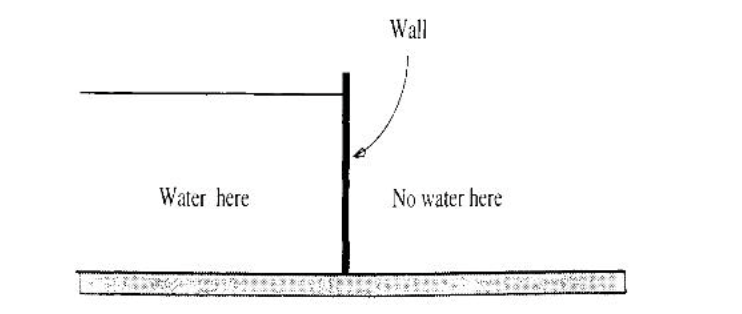
\includegraphics[width=0.7\linewidth]{images/dry-bed}
		\caption{ The Riemann problem with a dry bed (has no water) in one of the data state \cite{toro2001shock}.}
		\label{fig:dry-bed}
	\end{figure}
	
	\noindent There is only one rarefaction in the exact Riemann solution, that connects wet to dry state. The developing wet/dry interface is in this case single edge of the rarefaction, making it possible to determine the interface propagating speed using the corresponding characteristics field of the Riemann invariants \cite{ge:2008}.\\ 
	
	\noindent The wet/dry interface propagation  speed  is given by eqaution \eqref{wd0}, since the right state in figure \ref{fig:dry-bed}, is considered as the initial dry state, which also makes the rarefaction to be in the first characteristic field as shown in figure \ref{fig:wet-dry}.(a).
	
	\begin{equation}
		s_{i-\frac{1}{2}}^{3} = \check{s}_{i-\frac{1}{2}}^{+} = \lambda_{i-\frac{1}{2}}^{-*}(0)= U_{i-1} - 2\sqrt{gH_{i-1}}
		\label{wd0}
	\end{equation}
	
	\noindent If the left state in figure \ref{fig:dry-bed}, is considered as the initial dry state, then the  wet/dry interface propagation  speed  is given by eqaution \eqref{wd0}, and the  rarefaction is in the second characteristic field  as shown in figure \ref{fig:wet-dry}.(b).
	
	\begin{equation}
		s_{i-\frac{1}{2}}^{1} = \check{s}_{i-\frac{1}{2}}^{-} = \lambda_{i-\frac{1}{2}}^{+*}(0)= U_{i} - 2\sqrt{gH_{i}}
		\label{wd1}
	\end{equation}
	
	\begin{figure}[H]
		\centering
		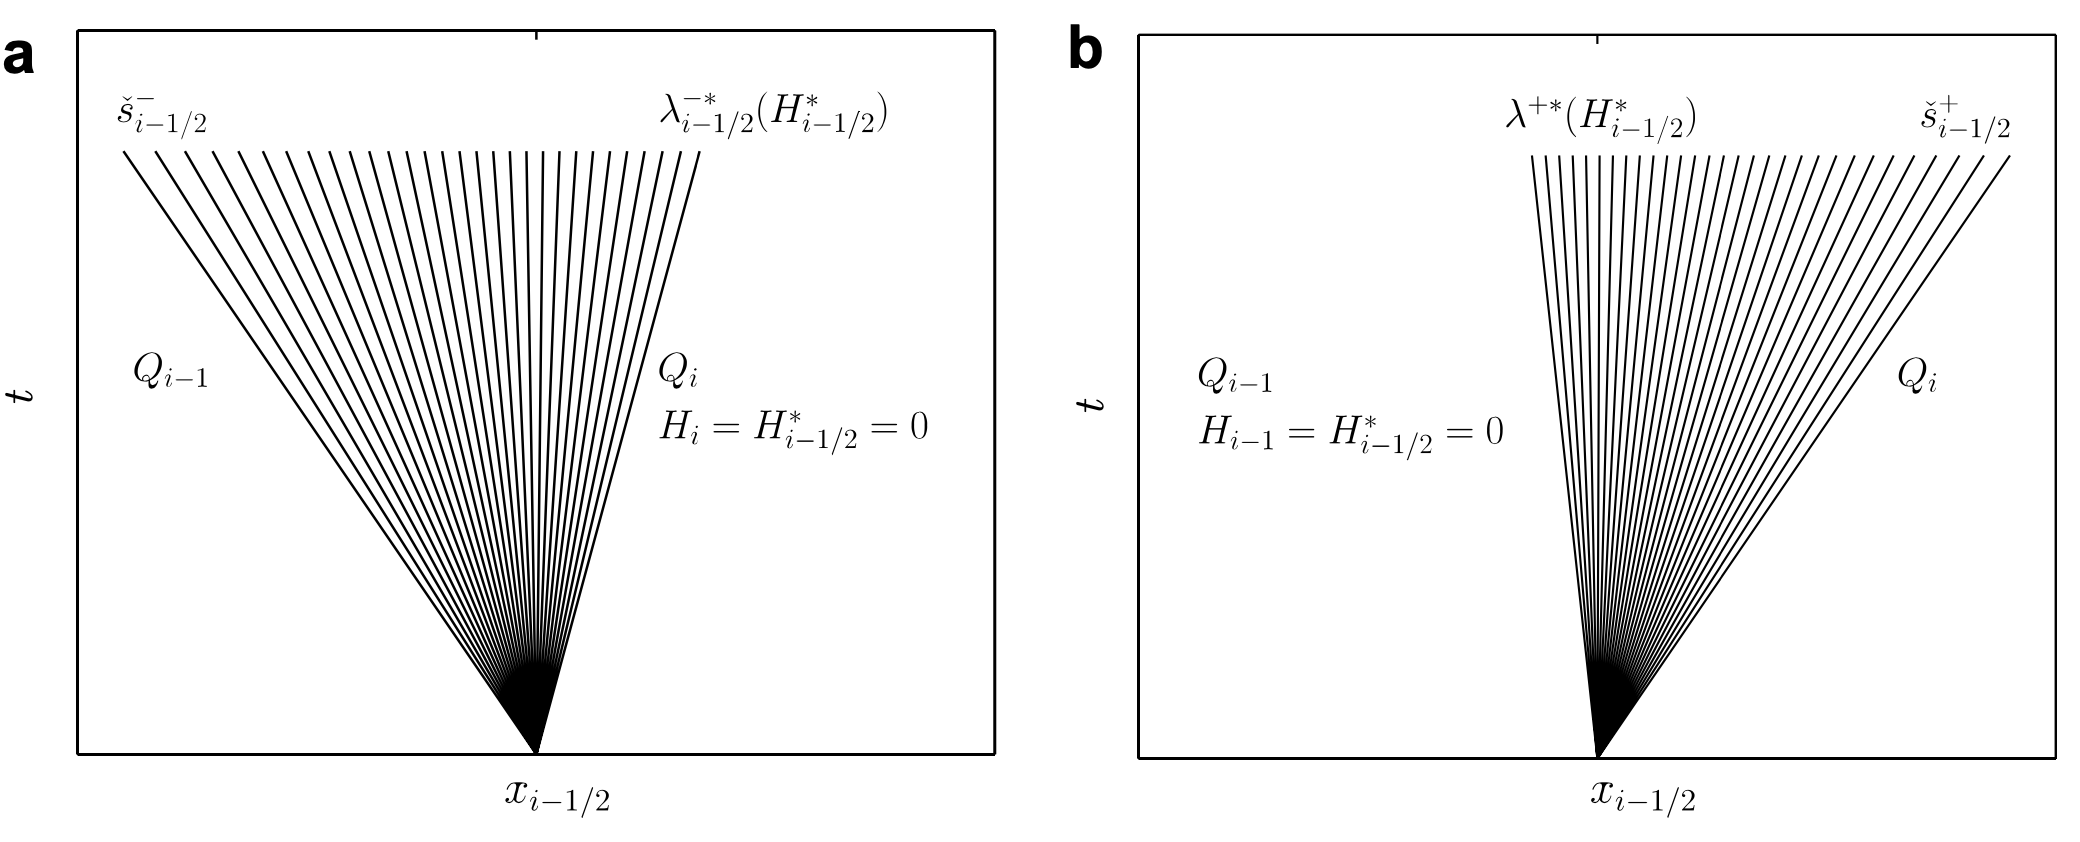
\includegraphics[width=.95\linewidth]{images/wet-dry}
		\caption{ The characteristic struture of  two dry intial state Riemann problem(dry bed) in the x-t plane \cite{ge:2008}.}
		\label{fig:wet-dry}
	\end{figure}
	
	
	
	\section{Numerical Examples}



	\bibliographystyle{plain}
	\bibliography{geoclaw}
	
\end{document}
